\documentclass[conference]{IEEEtran}

\usepackage{graphicx}
\usepackage{amsmath}
\usepackage{booktabs}
\usepackage{multirow}
\usepackage{cite}
\usepackage{url}

\title{Trustworthy Cardiac AI: Explainability, Domain Adaptation, and Clinical Workflow}

% \author{\IEEEauthorblockN{Author Name}
% \IEEEauthorblockA{Department\\University\\Email}}

\begin{document}
\maketitle

\begin{abstract}
% TODO: 150--250 words focusing on trust, deployment, and explainability.
\end{abstract}

\begin{IEEEkeywords}
Explainable AI; federated learning; ECG; domain adaptation; clinical workflow.
\end{IEEEkeywords}

\section{Introduction}
% Trustworthy AI motivation, clinical adoption challenges.

\section{Related Work}
% XAI in ECG, federated learning in healthcare, domain adaptation.

\section{System Overview}
\begin{figure}[t]
    \centering
    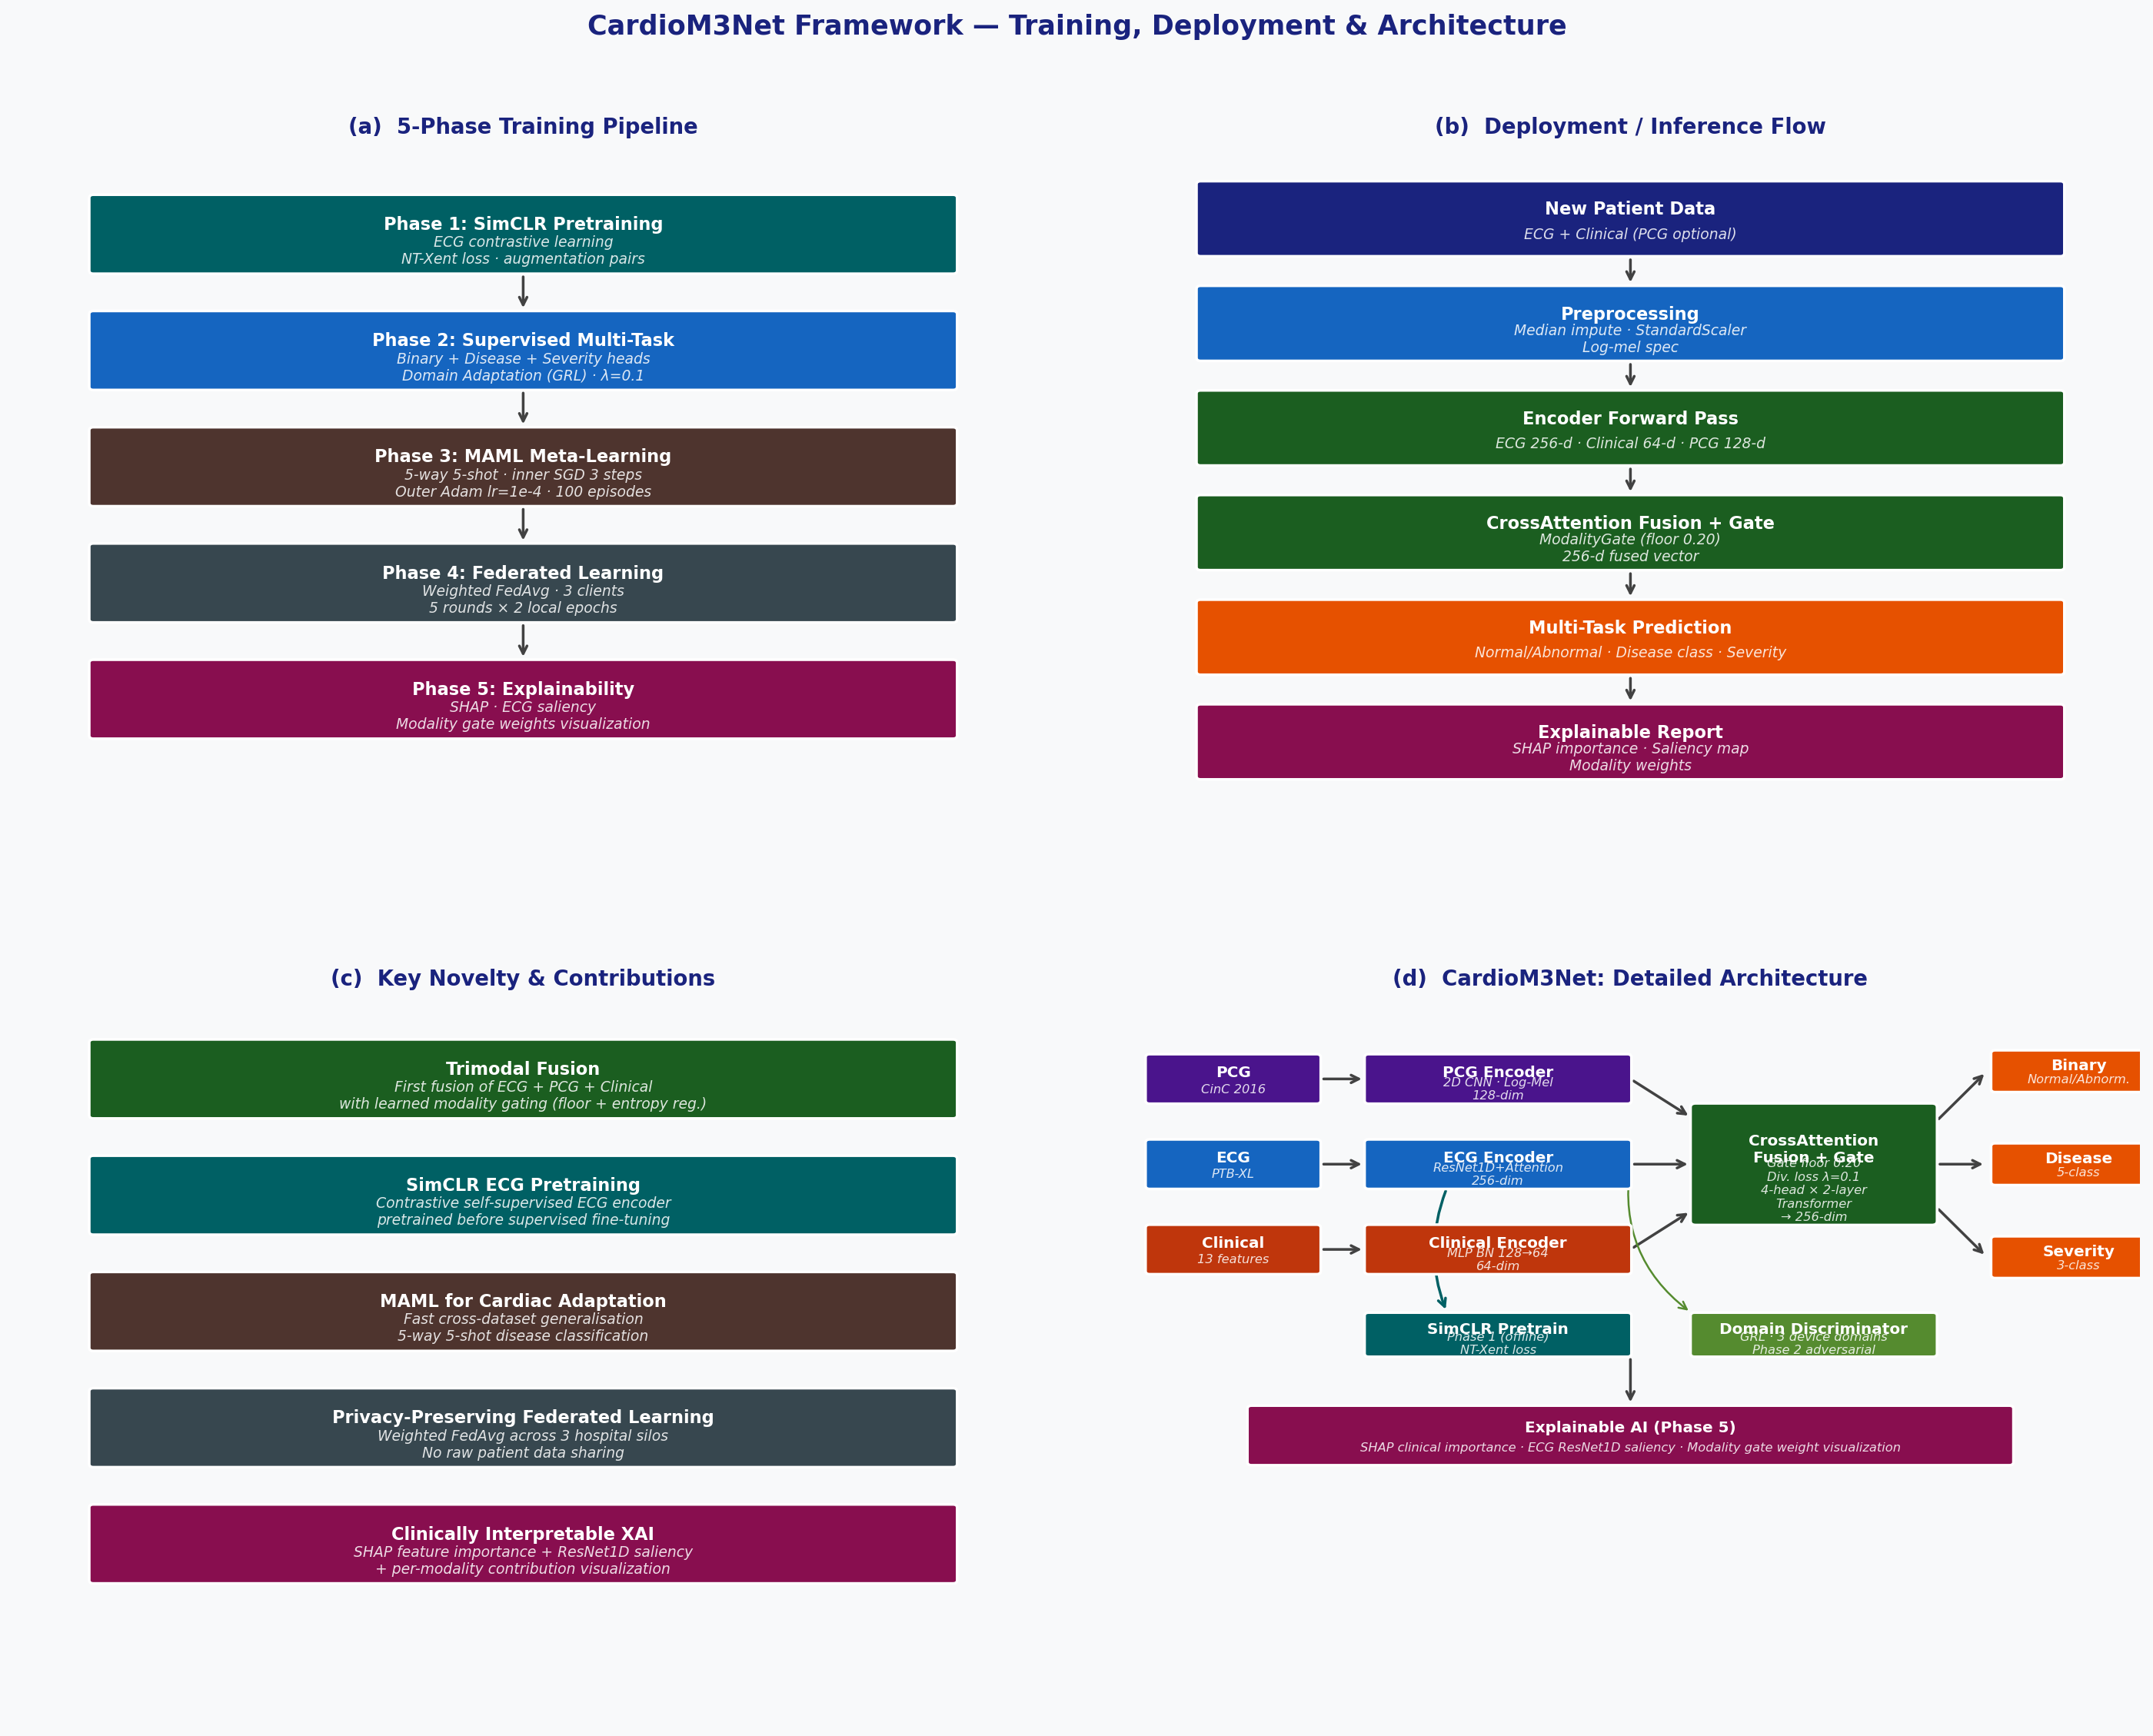
\includegraphics[width=\columnwidth]{../../cardiom3net_results/diagram2_pipeline.png}
    \caption{Training pipeline and deployment flow for CardioM3Net.}
    \label{fig:pipeline}
\end{figure}

\section{Methods}
\subsection{Domain Adaptation and Meta-Learning}
% GRL and MAML specifics.

\subsection{Federated Training}
% FedAvg configuration and privacy rationale.

\subsection{Explainability Stack}
% SHAP, Grad-CAM (1D), modality gates.

\section{Experiments}
% Evaluation protocol for explainability and deployment robustness.

\section{Results}
\subsection{Explainability}

\begin{figure}[t]
    \centering
    
\includegraphics[width=\columnwidth]{../../cardiom3net_results/ecg_saliency.png}
    \caption{1D Grad-CAM saliency for a single ECG sample showing diagnostically important time regions.}
    \label{fig:gradcam}
\end{figure}

\begin{figure*}[t]
    \centering
    
\includegraphics[width=\textwidth]{../../cardiom3net_results/ecg_saliency_grid.png}
    \caption{Grad-CAM saliency grid: one representative ECG per disease class with lead-weighted importance bars.}
    \label{fig:saliency_grid}
\end{figure*}

\begin{figure}[t]
    \centering
    
\includegraphics[width=\columnwidth]{../../cardiom3net_results/shap_clinical.png}
    \caption{SHAP summary (bar) showing mean absolute clinical feature importance.}
    \label{fig:shap}
\end{figure}

\begin{figure}[t]
    \centering
    
\includegraphics[width=\columnwidth]{../../cardiom3net_results/shap_clinical_detail.png}
    \caption{SHAP beeswarm plot showing directional impact of each clinical feature.}
    \label{fig:shap_detail}
\end{figure}

\begin{figure}[t]
    \centering
    
\includegraphics[width=\columnwidth]{../../cardiom3net_results/modality_weights.png}
    \caption{Average modality gate weights (ECG, Clinical, PCG) across the test set.}
    \label{fig:modality}
\end{figure}

\begin{figure}[t]
    \centering
    
\includegraphics[width=\columnwidth]{../../cardiom3net_results/modality_weight_distribution.png}
    \caption{Violin plots of per-sample modality gate weights stratified by disease class, revealing class-specific modality reliance.}
    \label{fig:modality_dist}
\end{figure}

\subsection{Performance and Robustness}
% Optionally include ROC or federated vs central comparison.

\begin{figure}[t]
    \centering
    
\includegraphics[width=\columnwidth]{../../cardiom3net_results/federated_convergence.png}
    \caption{Federated learning convergence: round-by-round binary accuracy, AUC, and disease accuracy compared to the centrally-trained baseline.}
    \label{fig:fed_conv}
\end{figure}

\begin{figure}[t]
    \centering
    
\includegraphics[width=\columnwidth]{../../cardiom3net_results/roc_curves.png}
    \caption{ROC curves for central and federated CardioM3Net (binary cardiac risk detection).}
    \label{fig:roc-b}
\end{figure}

\section{Discussion}
% Clinical interpretability and deployment considerations.

\section{Conclusion}
% Summary and next steps.

\section*{Acknowledgment}
% Optional.

\bibliographystyle{IEEEtran}
\bibliography{refs}

\end{document}
